In this chapter, we provide a proof of concept of Blockchain-based Federated Learning (BFS) applied to a system with vertically partitioned data. Specifically, we aim to:

\begin{enumerate}
    \item Present design and implementation of a Vertical Blockchain-based Federated Learning system. As discussed in \Cref{related_work:other_remarks}, only one other work \cite{10.48550/arxiv.1912.04859} discusses possibilities of integration of blockchain with Vertical Federated Learning with blockchain, but it does not provide an actual design or implementation.
    
    \item Demonstrate that our framework is flexible to support additional execution flow steps and algorithms, as well as both Horizontal and Vertical Federated Learning. As explained in \Cref{eval:ml_models}, the model we use for Vertical Federated Learning requires an additional step in each round. By showing that it is trivial to add new steps to the rounds, we also show that BlockLearning is flexible.
\end{enumerate}

\section{Requirements Analysis}

As discussed in \Cref{eval:ml_models}, our Vertical Federated Learning implementation uses the Split-CNN model. This model poses different requirements on our framework when compared to a regular CNN. These requirements are as follows:

\begin{enumerate}
    \item \textit{Support different models for the clients and the servers.} As explained in \Cref{eval:ml_models}, the clients have the head model, while the servers have the tail model. This is different than the model we used for Horizontal Federated Learning, which is the same on the devices, regardless of their type.
    
    \item \textit{Support additional backpropagation confirmation phase.} After submitting the aggregations, and before terminating the round, the clients have to confirm that they backpropagated the gradient updates from the tail model to their own head models. This is related to the fact that the clients and the servers have different models.
\end{enumerate}

The second requirement can be further divided into the following functional requirements:

\begin{enumerate}
    \item Execution of backpropagation confirmation phase after aggregations submission phase.
    \item Supporting backpropagation gradient submission by the servers to the smart contract.
    \item Supporting backpropagation retrieval by the clients from the smart contract.
    \item Supporting backpropagation confirmation by the clients to the smart contract.
\end{enumerate}

The execution flow of each round when a Split-CNN model is used is illustrated in \autoref{fig:steps_vertical}. Compared to the original execution flow, depicted in \autoref{fig:blocklearning_steps}, it becomes clear that (i) the scoring phase is not used, as it is not relevant in the context of Vertical Federated Learning, and (ii) there is an additional backpropagation confirmation phase before the round is terminated. 

\begin{figure}[!ht]
    \centering
    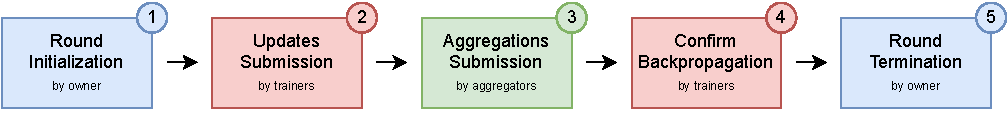
\includegraphics[width=1\textwidth]{graphics/sequence-vertical.pdf}
    \caption{Round Execution Flow With Split-CNN Model}
    \label{fig:steps_vertical}
\end{figure}

\section{BlockLearning's Extension}

Most of the aforementioned requirements pertain the smart contract. Therefore, we first start by making the required changes to the smart contracts:

\begin{enumerate}
    \item Add a new phase, called \texttt{WaitingForBackpropagation}, to the \texttt{RoundPhase} enumeration in the \texttt{Base} contract.
    
    \item Create a new smart contract, called \texttt{VerticalSplitCNN}, which inherits the main functionality from the \texttt{Base} smart contract, and provides the additional functionalities required for the backpropagation phase.
\end{enumerate}

\autoref{fig:uml-vertical} illustrates the smart contract additions to the original design of our BlockLearning framework presented in \Cref{chapter:framework}. It is important to note that all these changes are additions, and they do not change how any existing feature behaves.

\begin{figure}[!ht]
    \centering
    \centering
    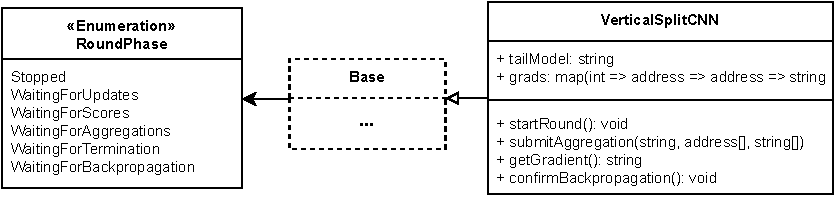
\includegraphics[width=1\textwidth]{graphics/smart-contract-uml-vertical.pdf}
    \caption{Split-CNN Smart Contracts Extension Class Diagram}
    \label{fig:uml-vertical}
\end{figure}

After creating the new smart contract, the smart contract bridge has to be extended in order to include the new smart contract functions. This extension is trivial as explained in \Cref{impl:bridge}.

The model training procedure for the Split-CNN model is slightly different from the CNN used for Horizontal Vertical Learning. For the Split-CNN, the clients submit an update with the intermediate outputs of the last layer of the head model, instead of the weights. During the aggregation phase, the servers calculate the gradients of the intermediate outputs, which are then backpropagated to the clients. To support this, we implement two new classes: \texttt{TrainerSplitCNN} and \texttt{AggregatorSplitCNN}, which implement the \texttt{trainer()} and \texttt{aggregate()} interfaces, respectively, as specified in \Cref{chapter:framework}. In addition, the \texttt{TrainerSplitCNN} class supports a new method, \texttt{backward()}, that will be called during the new backpropagation phase.

Finally, we write server and client scripts for the Vertical Federated Learning using the building blocks from the BlockLearning framework. \autoref{alg:client_loop_splitcnn} illustrates the client main loop when used with a Split-CNN model. The main differences from the original BlockLearning framework, as presented in \Cref{chapter:framework}, are that the framework does not have scoring algorithm, and that we take into account the backpropagation phase. The server main loop when used with a Split-CNN model is the same as the original server main loop except that it initializes an instance of the \texttt{AggregatorSplitCNN} class instead of the regular aggregator.

\begin{algorithm}
\caption{Client Script Main Loop for Split-CNN}\label{alg:client_loop_splitcnn}
\begin{algorithmic}
\State $T \gets $ Initialize Split-CNN Trainer
\While{True}
    \State $P \gets$ Get Phase From Smart Contract
    \If{$P$ is Waiting For Updates}
        \State Execute Training Procedure $T.train()$
    \ElsIf{$P$ is Waiting For Backpropagation}
        \State Execute Backpropagation Procedure $T.backward()$
    \EndIf
\EndWhile
\end{algorithmic}
\end{algorithm}

\section{Experiments and Results}

After extending our framework in order to support the Split-CNN model, we executed the experiments for Vertical Federated Learning in order to validate whether our implementation was successful and the Vertical BFL can be supported. The experiments were executed in the same way as the experiments for the Horizontal BFL, using BlockLearning's Testbed. The only difference is that, this time, we used the client and server scripts that we developed for the Split-CNN model.

We ran two experiments with two different number of clients: 2 and 4. The decision to use 2 clients was motivated by \cite{10.1145/3297858.3304038}, where the Split-CNN was introduced for Vertical FL without blockchain for the first time. In addition, we also performed experiments with 4 clients.

\subsection{Execution Time, Transaction Cost, and Transaction Latency}

As it can be seen from \autoref{tab:metrics_vertical}, this experiment was faster than most experiments, which is easily explained by the low number of clients. In addition, it is observed that the experiments take longer with 4 clients than with 2.

Regarding the transaction latency, it can be seen that it is similar to what we have seen in previous chapters. Similarly, the transaction costs do not present significant changes as the number of clients is relatively low. However, as expected, the transaction costs are slightly higher in case of having 4 clients.

\begin{table}[!ht]
\begin{tabular}{c|c|c} \hline \hline
                                & 2             & 4             \\ \hline \hline
E2E Time (m)                    & 18.08         &	24.30       \\ \hline
Mean Round Time (s)             & 21.68         &	29.15       \\ \hline
Mean Transaction Latency (s)    & 1.482         &	1.418       \\ \hline
Mean Transaction Cost (Gas)     & 138659        &	141013      \\ \hline
\end{tabular}
\caption{Execution Time, Transaction Cost, and Transaction Latency Per Number of Clients}
\label{tab:metrics_vertical}
\end{table}

\subsection{Model Accuracy and Convergence}

\autoref{fig:accuracy_vertical} illustrates the model accuracy of our experiments as well as those of Romanini et al. \cite{10.48550/arxiv.2104.00489}, where a Split-CNN model without blockchain was used with the MNIST data set. It can be seen that model accuracy of \cite{10.48550/arxiv.2104.00489} is higher, which may be related to implementation differences such as the Machine Learning library used, which is not known.

\begin{figure}[!ht]
    \centering
    \centering
    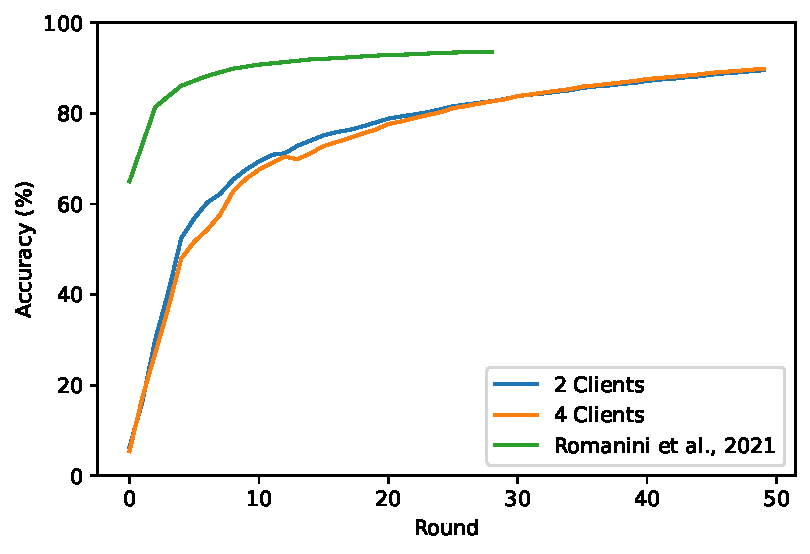
\includegraphics[width=0.7\textwidth]{graphics/vertical/accuracy.pdf}
    \caption{Model Accuracy Per Number of Clients}
    \label{fig:accuracy_vertical}
\end{figure}

\subsection{Communication Costs}

The communication costs, illustrated in \autoref{fig:net_vertical}, are also within the expected values.

We can observe at the client sides that there is no major difference of traffic when the number of clients increases. This can be explained by the fact that, by using a Split-CNN, each client is only required to upload its own intermediate results and downloads the gradient updates, which are similar in size.

At the servers, the costs are higher as the number of clients increases. Since the higher number of clients lead to higher number of heads in the Split-CNN model, the servers are required to download more intermediate results and to upload more gradient updates. Therefore, the network traffic at the servers increases with the number of clients.

On the blockchain, the difference of number of clients is not significant to make a significant difference on traffic, since these experiments ran with a very low number of clients.

\begin{figure}[!ht]
    \centering
    \centering
    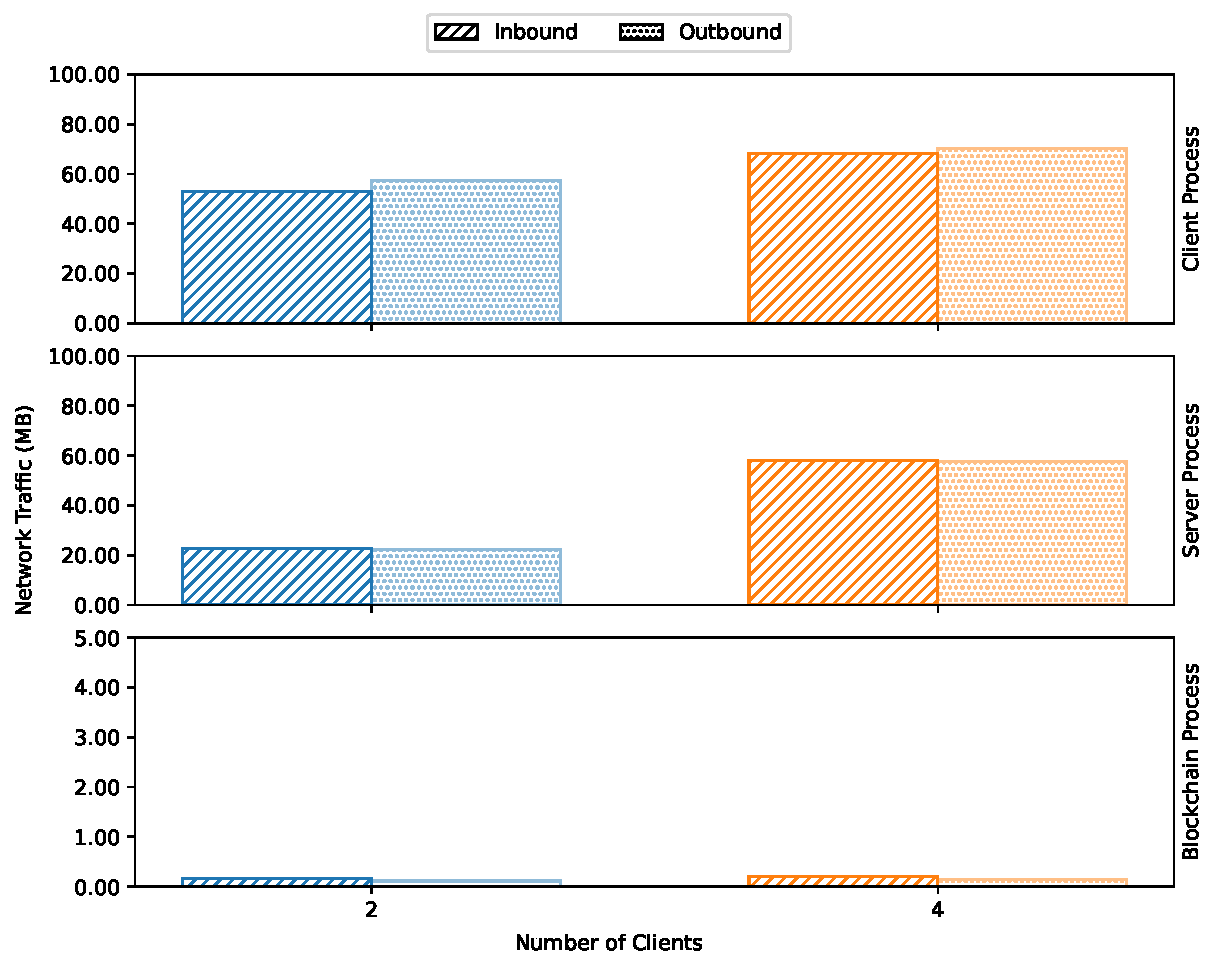
\includegraphics[width=0.8\textwidth]{graphics/vertical/net.pdf}
    \caption{Network Traffic Per Round Per Number of Clients}
    \label{fig:net_vertical}
\end{figure}

\subsection{Computation Costs}

Computation costs, namely RAM usage and CPU usage, are depicted in \autoref{fig:ram_vertical} and \autoref{fig:cpu_vertical}, respectively.

Regarding the RAM usage, we observe that with a higher number of clients, there is a higher RAM usage on the serves and the blockchain processes. This is caused by the fact that more data is being stored in-memory due to the higher amount of intermediate results that the servers store in-memory, as well as the number of blockchain transactions in the blockchain. At the clients, however, the opposite happens. This can be explained by the fact that when there are more clients, each client has less features as per the data partitioning explained in \Cref{eval:client_sampling}.

Regarding the CPU usage, we see similar results as to the RAM usage, which are explained by the same reasons.

\section{Conclusions and Improvements}

From our experiments, we can conclude that it is possible to apply a Blockchain-based Federated Learning system to vertically partitioned data. In addition, we also showed how flexible our BlockLearning framework is and how we can add new features to it without changing the rest of the framework.

In future, it would be interesting to investigate how to make BlockLearning more generic in order to support other Vertical Federated Learning models than only Split-CNN. In addition, it would be interesting to incorporate the Private Set Intersection phase into our framework. This would allow the framework to be directly applied to cases where the clients have intersecting, but not equal, sample spaces.

\clearpage

\begin{figure}[!hpt]
    \centering
    \centering
    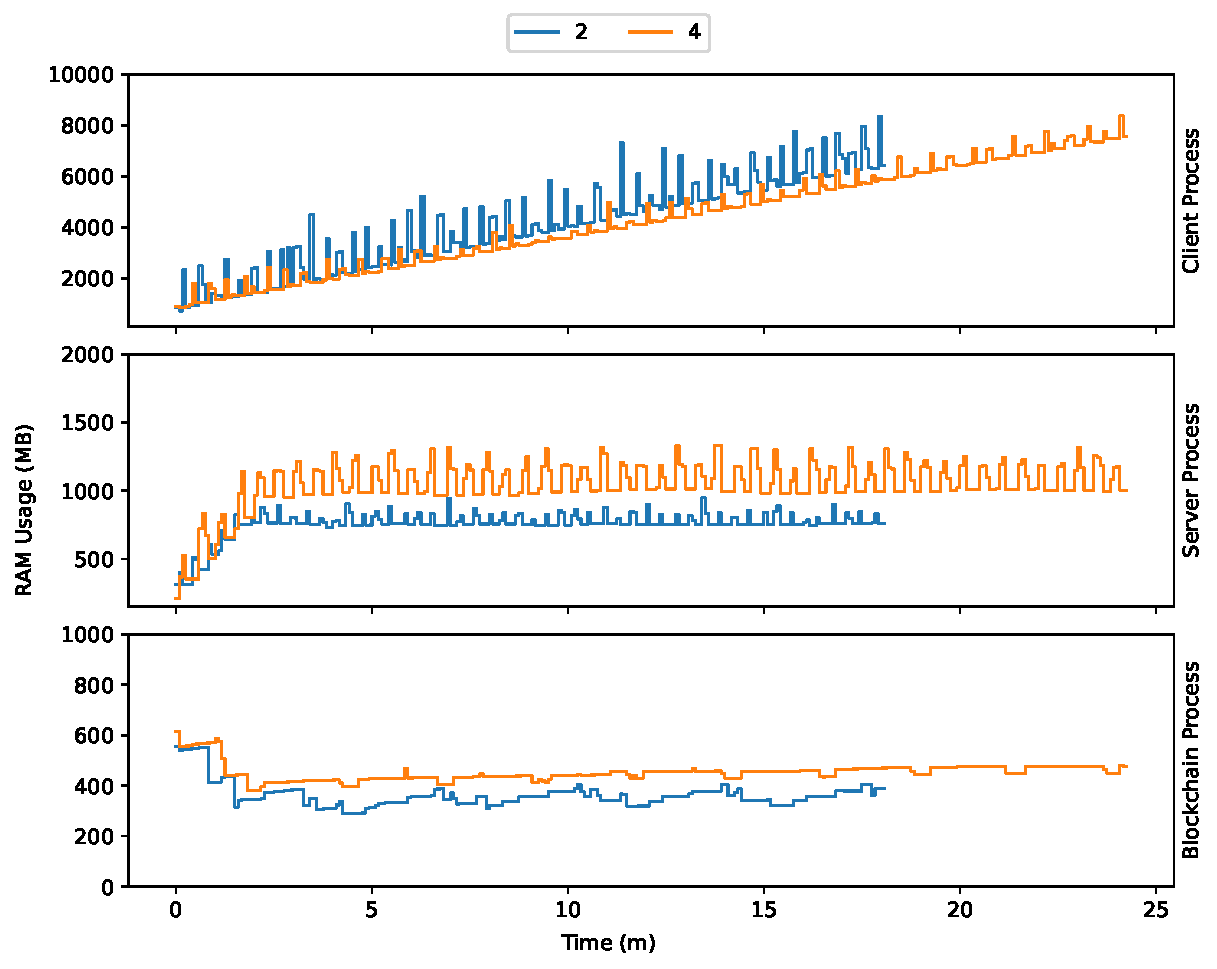
\includegraphics[width=0.8\textwidth]{graphics/vertical/ram.pdf}
    \caption{RAM Usage Per Number of Clients}
    \label{fig:ram_vertical}
\end{figure}

\begin{figure}[!hpb]
    \centering
    \centering
    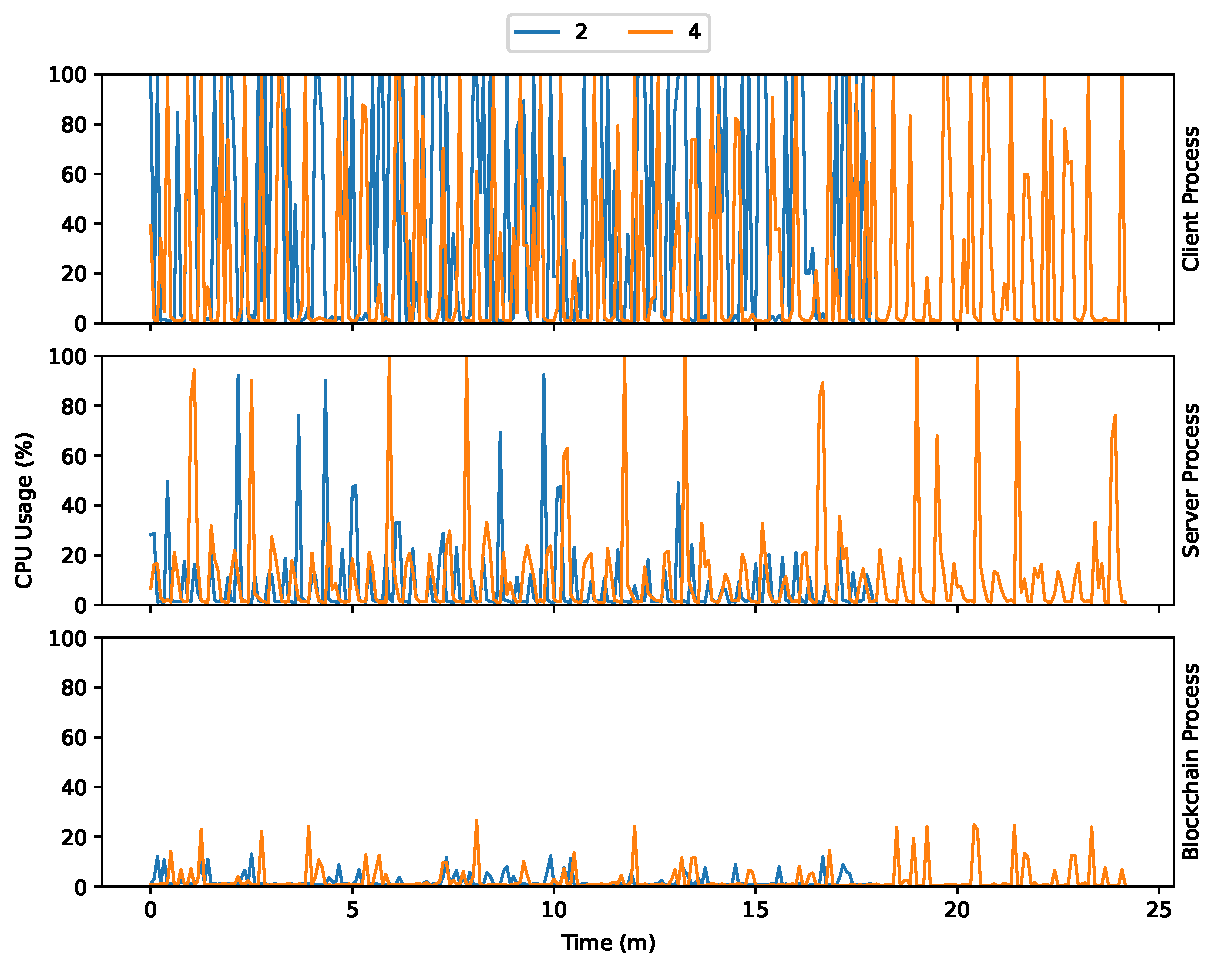
\includegraphics[width=0.8\textwidth]{graphics/vertical/cpu.pdf}
    \caption{CPU Usage Per Number of Clients}
    \label{fig:cpu_vertical}
\end{figure}